\documentclass{beamer}

% Prévoir à peu près un transparent par minute d'exposé.
% Deux ou trois sections semble être une bonne chose.


\usepackage[french]{babel}
\usepackage[utf8]{inputenc}
\usepackage{times}
\usepackage{verbatim}
\usepackage[T1]{fontenc}
\usepackage{listings}
\RequirePackage[lined,boxed,commentsnumbered]{algorithm2e}
\usepackage{monTheme4}

\begin{document}

\begin{frame}
  % Insertion du logo
   \begin{center}
     
\includegraphics[width=0.2\textwidth]{logo/logo.png}
   \end{center}
  \titlepage
\end{frame}

%%%%%%%%%%%%%%%%%%%%%%%%%%%%%%%%%%%%%%%%%%%%%%%%%%%%%%%%%%%%%%%%%%%%%%%%%%%%%%%%%%%%%%%%%%%%%%%%%%%%%%

\section*{Introduction}

\begin{frame}
  \frametitle{Introduction}

  \begin{block}{Le nucléole}
    \begin{itemize}
    \item Localisation nucléaire 
    \item Encore mal connu
    \item Responsable de certaines pathologies
    \item Peu d'outils pour l'étude \textit{in silico}
    \end{itemize}
  \end{block}

  \begin{block}{NuQleoSim}
    \begin{itemize}
    \item Interface graphique pour l'étude du nucléole
    \item Base de données : moléculaires et expérimentales
    \item Modélisation de l'activité nucléolaire
    \item Gestion des résultats
    \end{itemize}
  \end{block}

\end{frame}

\begin{frame}
  \frametitle{Plan}
  \tableofcontents
\end{frame}

%%%%%%%%%%%%%%%%%%%%%%%%%%%%%%%%%%%%%%%%%%%%%%%%%%%%%%%%%%%%%%%%%%%%%%%%%%%%%%%%%%%%%%%%%%%%%%%%%%%%%%%%%%%

\section{Analyse}

\subsection{Contexte biologique : le nucléole}

\begin{frame}
  
  \begin{block}{Structure du nucléole en microscopie électronique}

    \begin{center}
      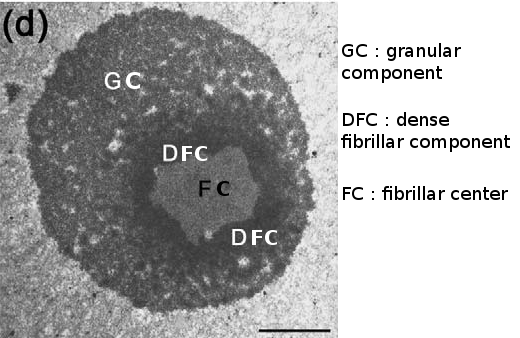
\includegraphics[width=0.6\textwidth]{img/microNuc.png}
    \end{center}

    
    Ivan Raska, Peter J Shaw, and Dusan Cmarko. \textit{Structure and function of the nucleolus in the spotlight.} Curr Opin Cell Biol, Jun 2006.
  \end{block}

\end{frame}

\begin{frame}
  
  \begin{block}{Biogénèse des ribosomes}
  \begin{center}
    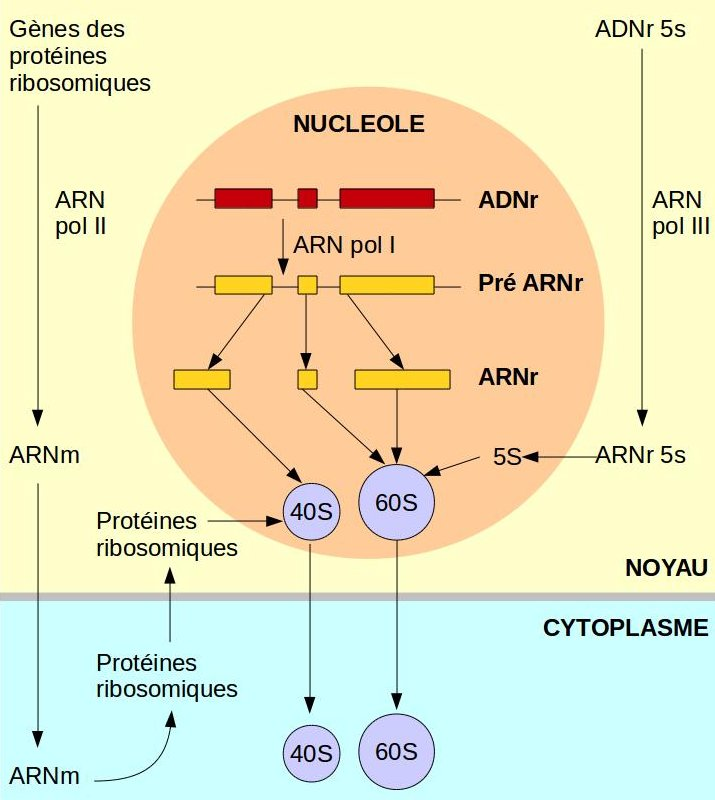
\includegraphics[width=0.5\textwidth]{img/biogenese.png}
  \end{center}
  \end{block}

\end{frame}

\subsection{Besoins fonctionnels et non fonctionnels}

\begin{frame}
  \begin{center}
    
\includegraphics[width=0.2\textwidth]{img/db.png}
  \end{center}
  
  \bigskip  
  
  \begin{block}{Stockage de données}
    \begin{itemize}
    \item Deux types de données : moléculaires et expérimentales
    \item Création, consultation, modification et suppression
    \item Interopérabilité avec différents formats biologiques
    \end{itemize}
  \end{block}
\end{frame}

\begin{frame}
  \begin{center}
    
\includegraphics[width=0.3\textwidth]{img/rouages.png}
  \end{center}
  
  \bigskip  
  
  \begin{block}{Modélisation de l'activité nucléolaire}
    \begin{itemize}
    \item Interface de paramétrage de la simulation
    \item Communication avec la base de données
    \item Visualisation 3D en temps réel
    \item Génération de résultats
    \end{itemize}
  \end{block}

\end{frame}

%%%%%%%%%%%%%%%%%%%%%%%%%%%%%%%%%%%%%%%%%%%%%%%%%%%%%%%%%%%%%%%%%%%%%%%%%%%%%%%%%%%%%%%%%%%%%%%%%%%%%%

\section{Conception}

\subsection{Base de données nucléolaires}

\begin{frame}
  \begin{block}{Organisation de la base de données}
  \begin{center}
    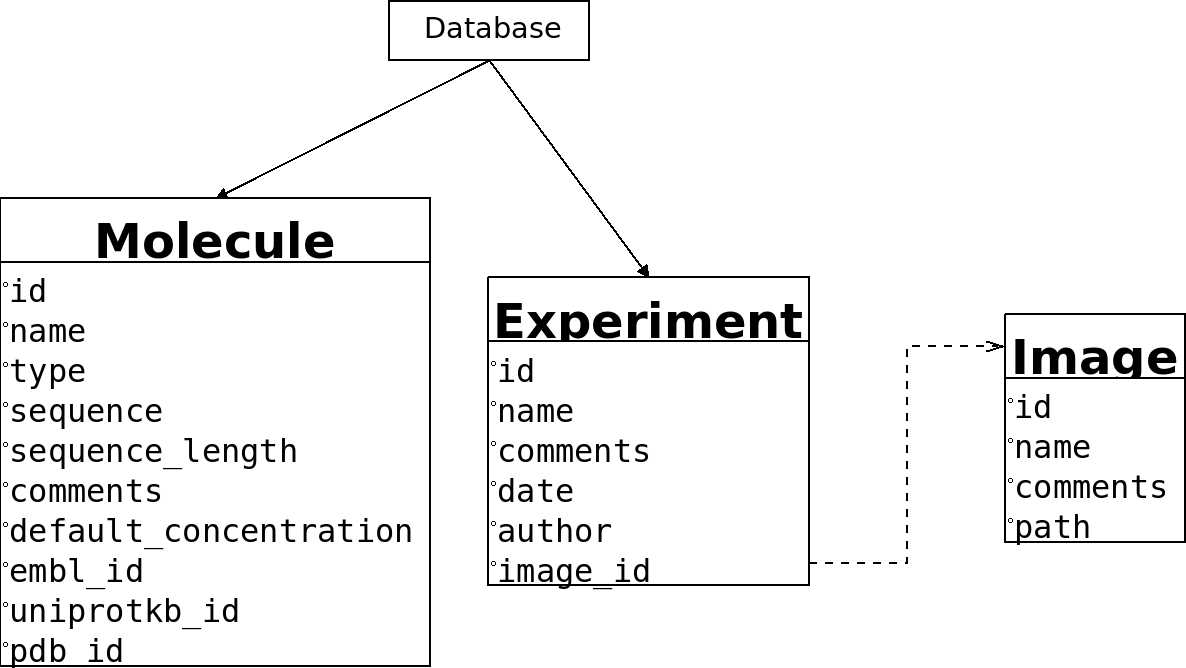
\includegraphics[width=0.9\columnwidth]{img/diagDB.png}
  \end{center}
  \end{block}
\end{frame}

\subsection{Modélisation du nucléole}

\begin{frame}
	\frametitle{Utilisation d'un système multi-agents}
	\begin{block}{Environnement}
		\begin{itemize}
			 \item nucléole
			 \item subdivision en trois composants
			 \begin{itemize}
			 	\item FC
			 	\item DFC
			 	\item GC
			\end{itemize}
		\end{itemize}
  	\end{block}
  	\begin{block}{Agents}
		\begin{itemize}
			 \item protéine
			 \item " transcriptor "
			 \item ARN
		\end{itemize}
  	\end{block}
\end{frame}

\begin{frame}
  \begin{block}{Règles d'intéractions des agents}
  \begin{center}
    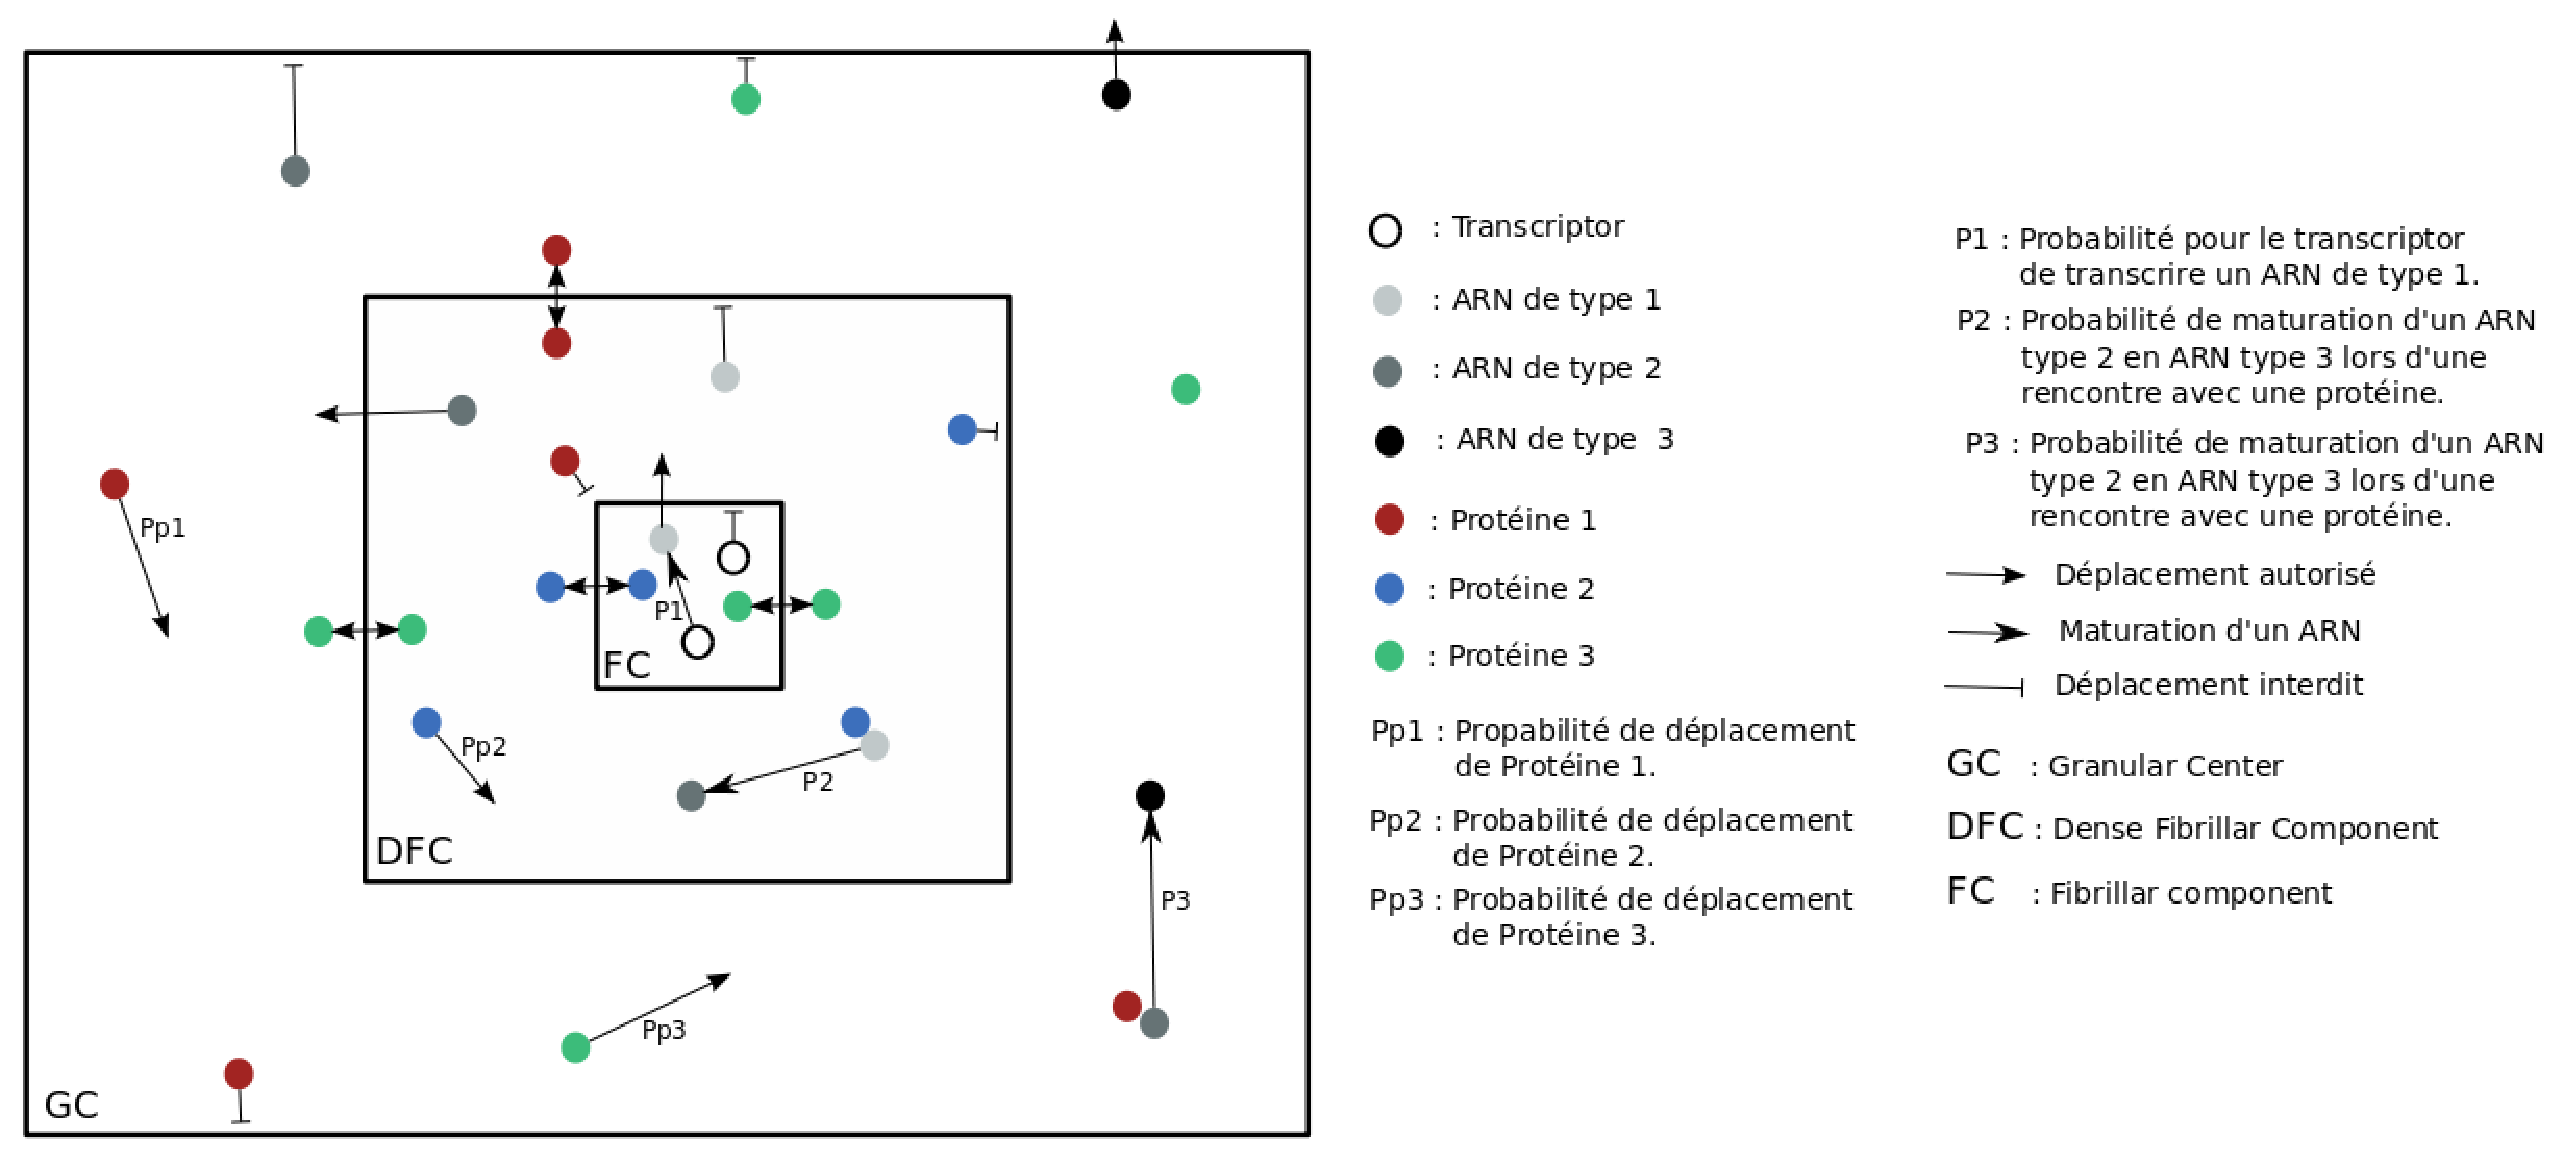
\includegraphics[width=1\columnwidth]{img/schemaSimu.pdf}
  \end{center}
  \end{block}
\end{frame}

\subsection{Prototypage de l'interface}

\begin{frame}

  \begin{block}{Premier modèle envisagé}
  \begin{center}
    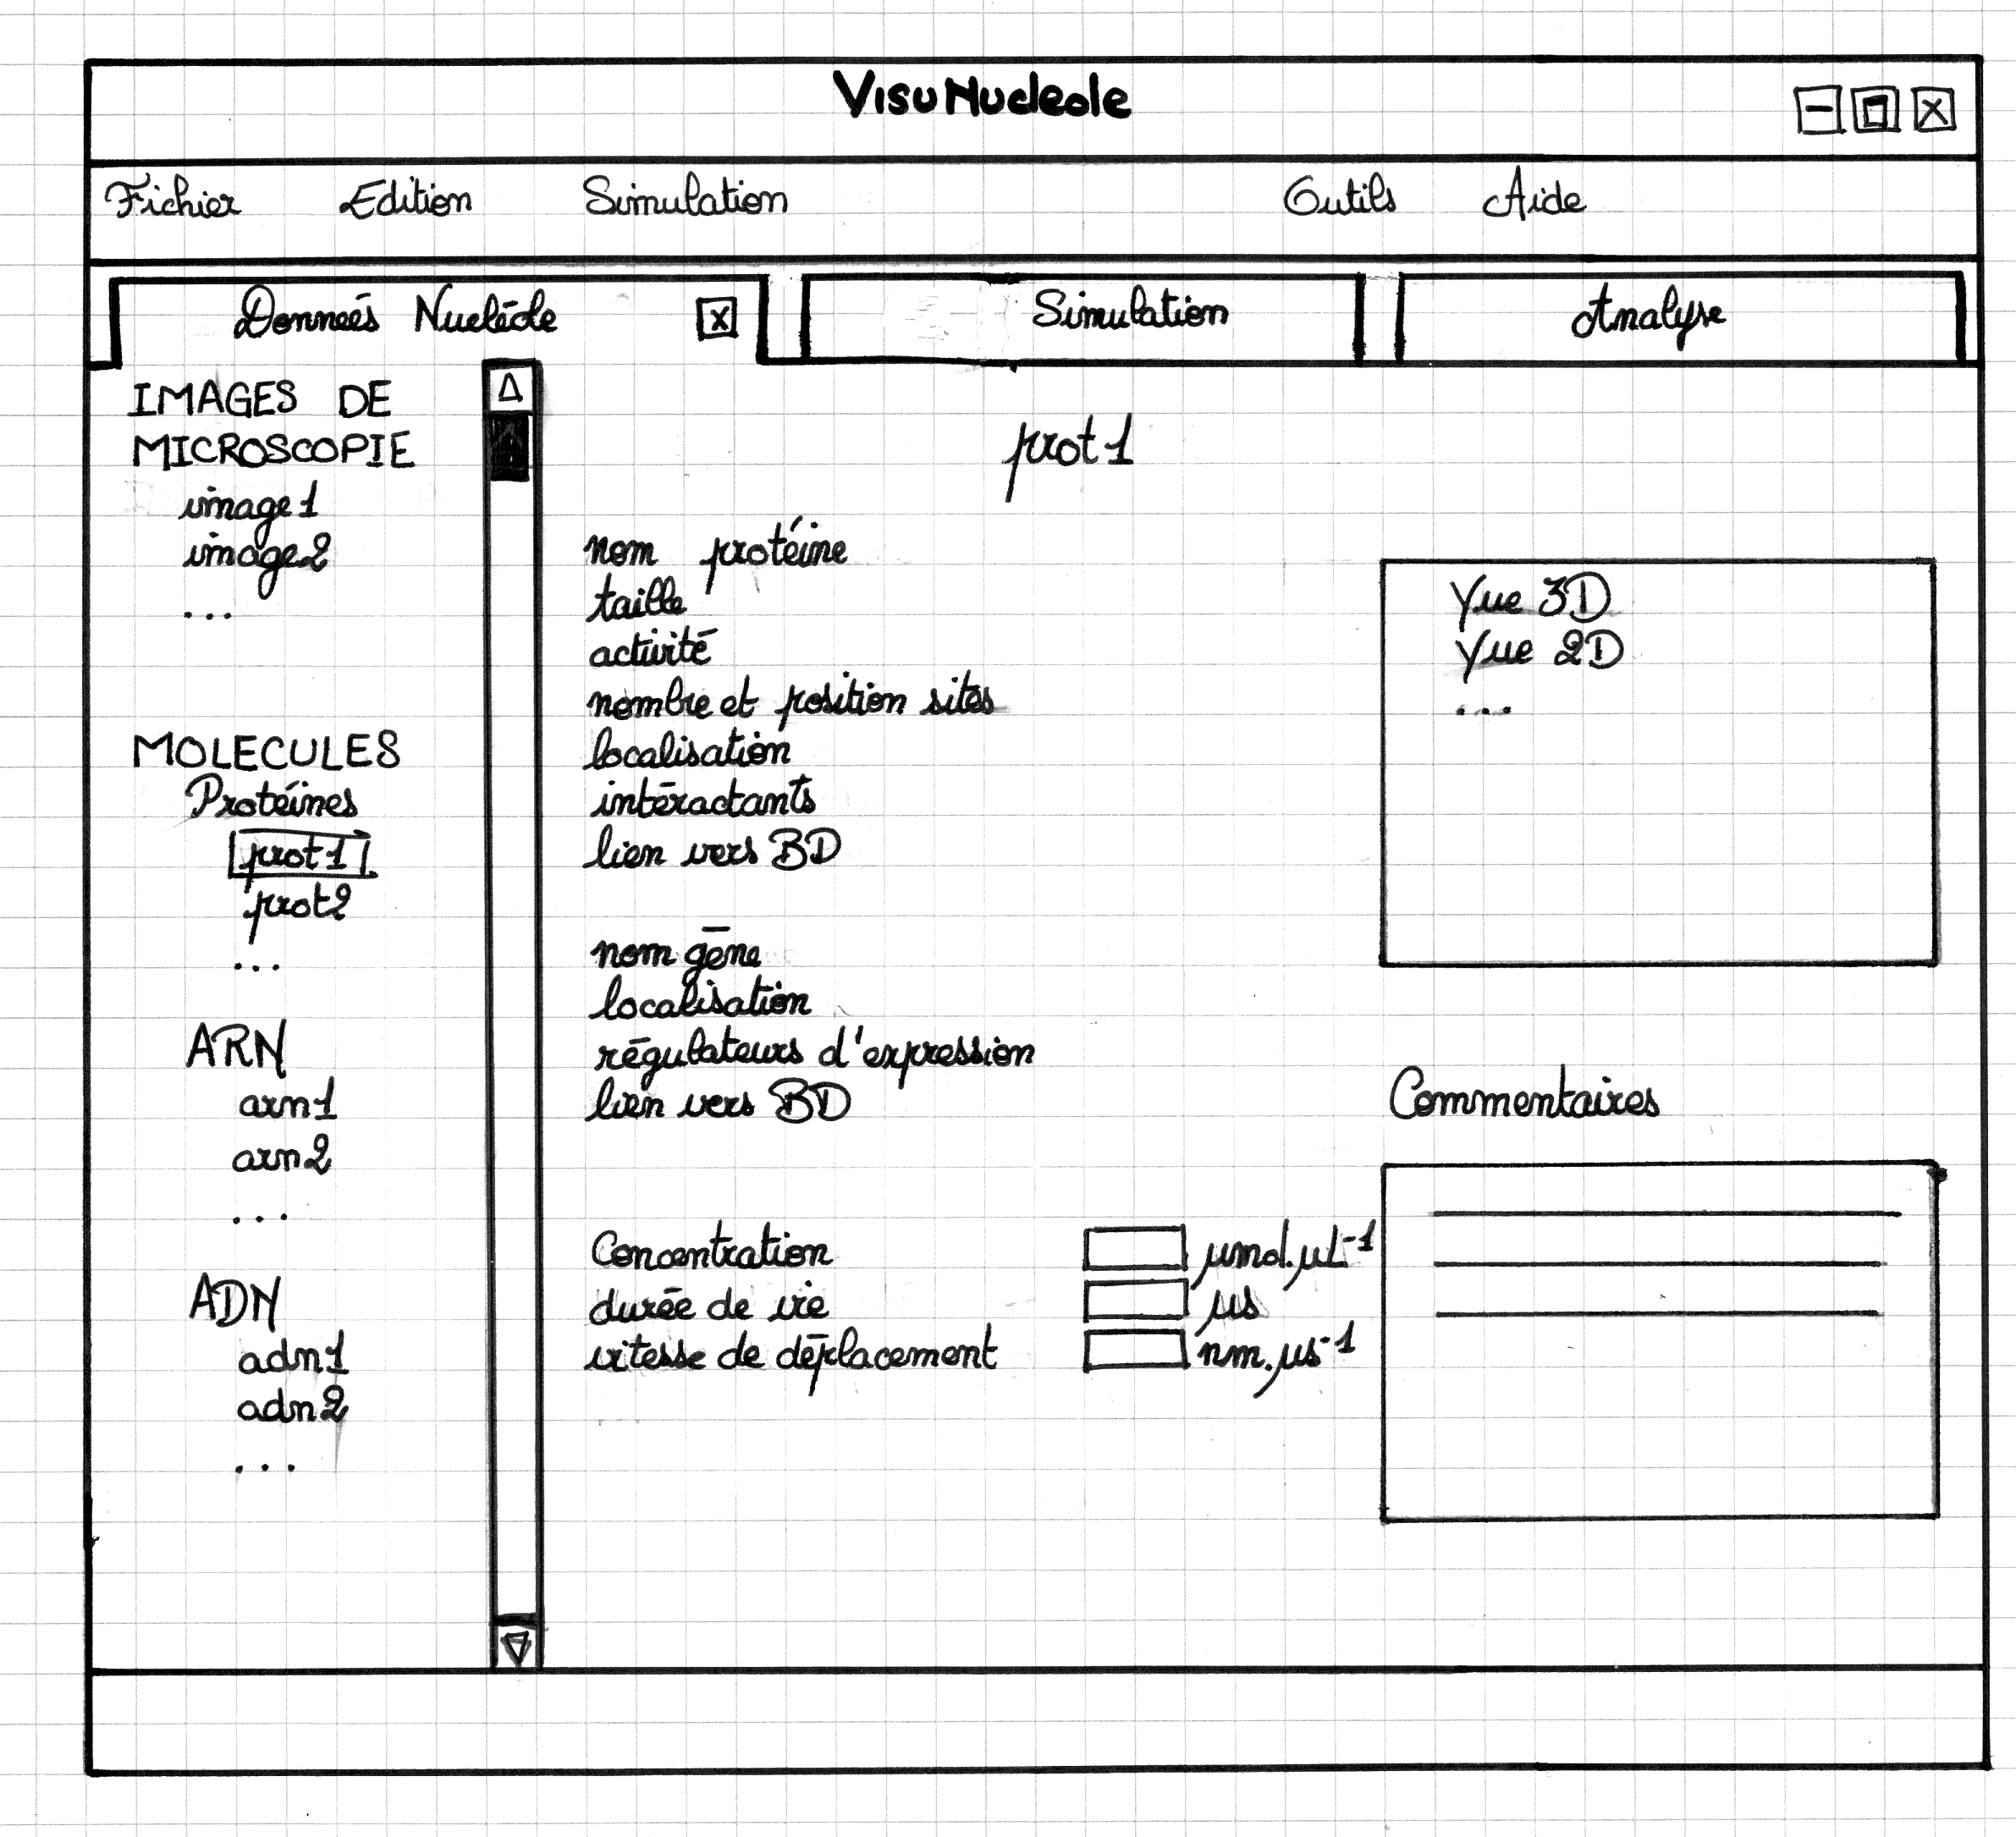
\includegraphics[width=0.7\columnwidth]{img/mock1.png}
  \end{center}
  \end{block}

\end{frame}

%%%%%%%%%%%%%%%%%%%%%%%%%%%%%%%%%%%%%%%%%%%%%%%%%%%%%%%%%%%%%%%%%%%%%%%%%%%%%%%%%%%%%%%%%%%%%%%%%%%%%%

\section{Réalisation}

\subsection{Technologies utilisées}

\begin{frame}

  \begin{center}
    
\includegraphics[width=0.3\textwidth]{img/qt-logo.png}
  \end{center}

  \begin{block}{Qt / C++}
    \begin{itemize}
    \item Performances de calcul
    \item Qt en tant que framework : 
      \begin{itemize}
      \item Multiplateforme
      \item Rapidité de développement
      \end{itemize}
    \end{itemize}
  \end{block}
\end{frame}

\begin{frame}
  \frametitle{Système de Gestion des Bases de Données}

  \begin{block}{Architecture modulable}
    \begin{itemize}
    \item Possibilité d'ajouter des interfaces à des SGBD
    \end{itemize}
  \end{block}

  \begin{block}{Pourquoi XML comme SGBD ?}
    \begin{itemize}
    	\item Léger :  ne nécessite pas de serveur
    	\item Format répandu : nombreuses bibliothèques
    	\item Inconvénients : 
    	\begin{itemize}
    		\item cas de la gestion de grandes BD
    		\item droits d'accès
    	\end{itemize}
    \end{itemize}
  \end{block}

\end{frame}

\subsection{Structuration de la base de données}

\begin{frame}
  \begin{block}{Arborescence du fichier XML}
  \begin{center}
    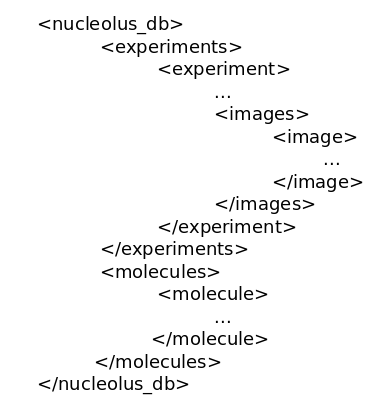
\includegraphics[width=0.4\columnwidth]{img/xmlBD.png}
  \end{center}
  \end{block}
\end{frame}

\subsection{Architecture de l'application}

\begin{frame}

  \begin{block}{Diagramme de classe}
  \begin{center}
      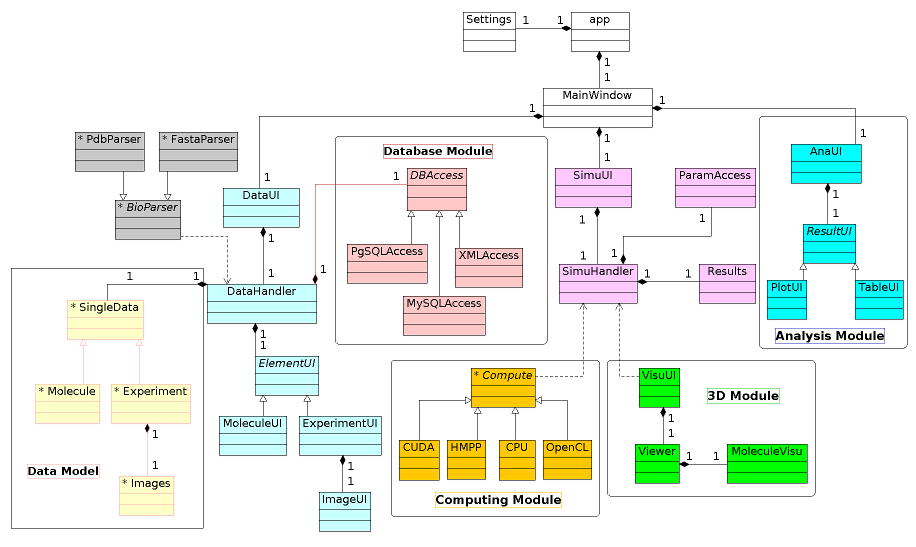
\includegraphics[width=1\columnwidth]{img/diag.png}
  \end{center}
  \end{block}

\end{frame}



\subsection{Implémentation de la modélisation}

\begin{frame}
  \begin{block}{Structure du système multi-agents}
  \begin{center}
    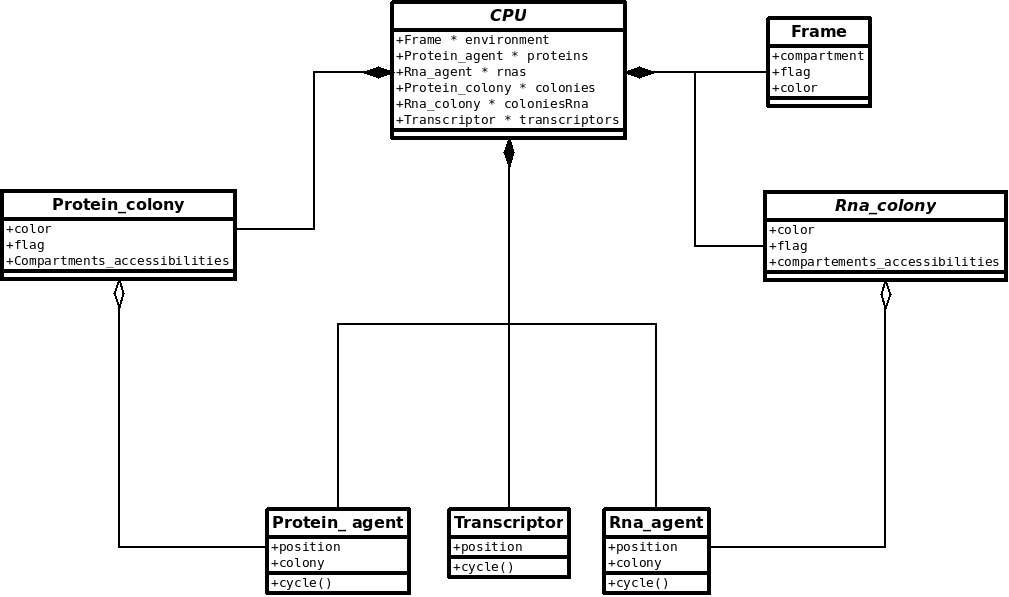
\includegraphics[width=1\columnwidth]{img/diag_SMA.png}
  \end{center}
  \end{block}
\end{frame}

%%%%%%%%%%%%%%%%%%%%%%%%%%%%%%%%%%%%%%%%%%%%%%%%%%%%%%%%%%%%%%%%%%%%%%%%%%%%%%%%%%%%%%%%%%%%%%%%%%%%%%%%%%%%%%

\section{Résultats}

\subsection{Interface avec la base de données}

\begin{frame}
  \begin{center}
      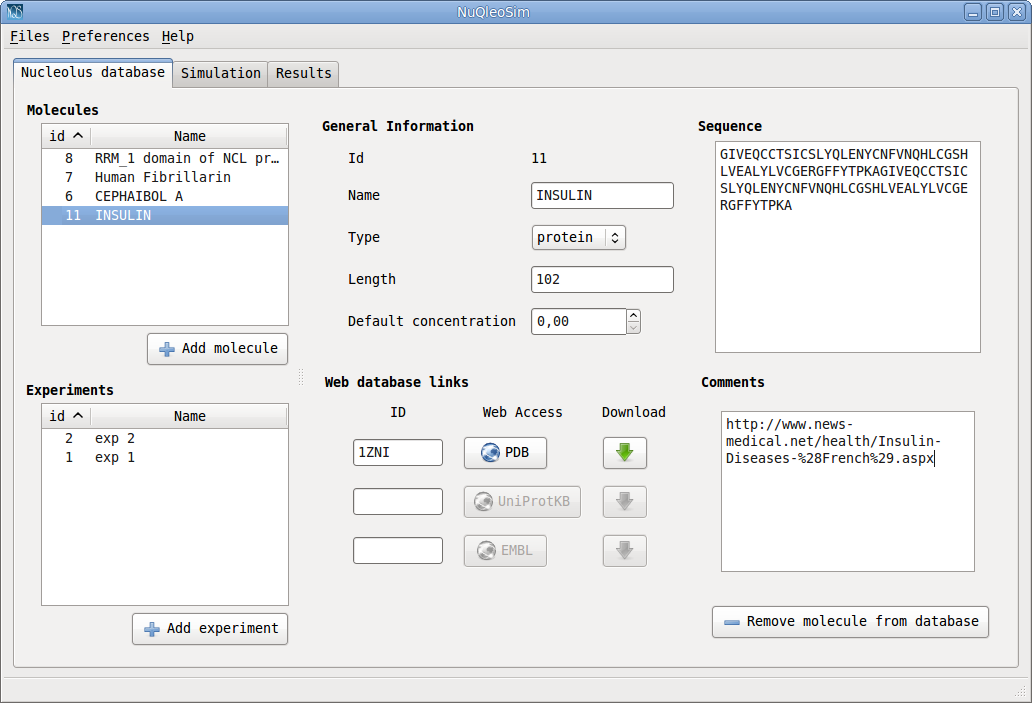
\includegraphics[width=0.9\columnwidth]{img/inter1.png}
  \end{center}
\end{frame}

\subsection{Paramétrage d'une simulation}
\begin{frame}
  \begin{center}
      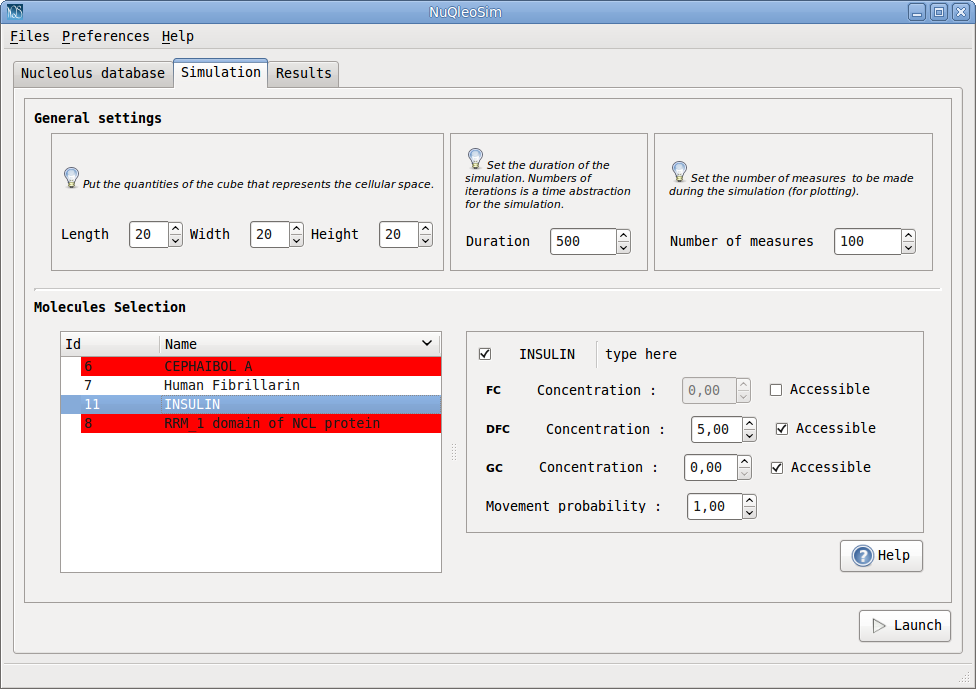
\includegraphics[width=0.9\columnwidth]{img/inter2.png}
  \end{center}
\end{frame}

\subsection{Visualisation de la modélisation}
  
\begin{frame}
    \begin{center}
      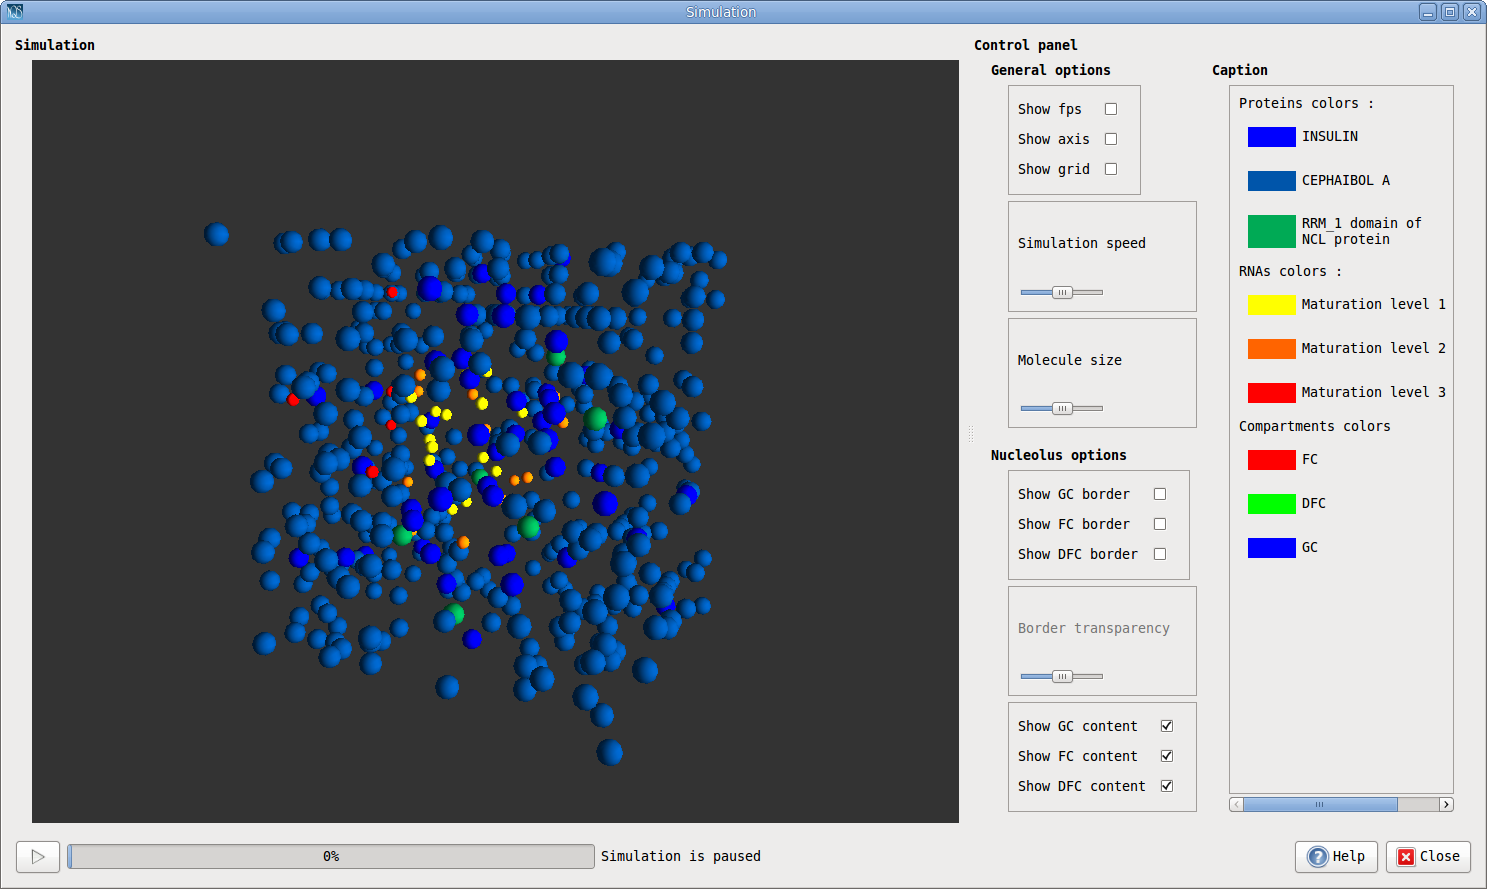
\includegraphics[width=1\columnwidth]{img/inter3.png}
  \end{center}
\end{frame}

\subsection{Exemple de génération de résultats}
\begin{frame}
  \begin{center}
      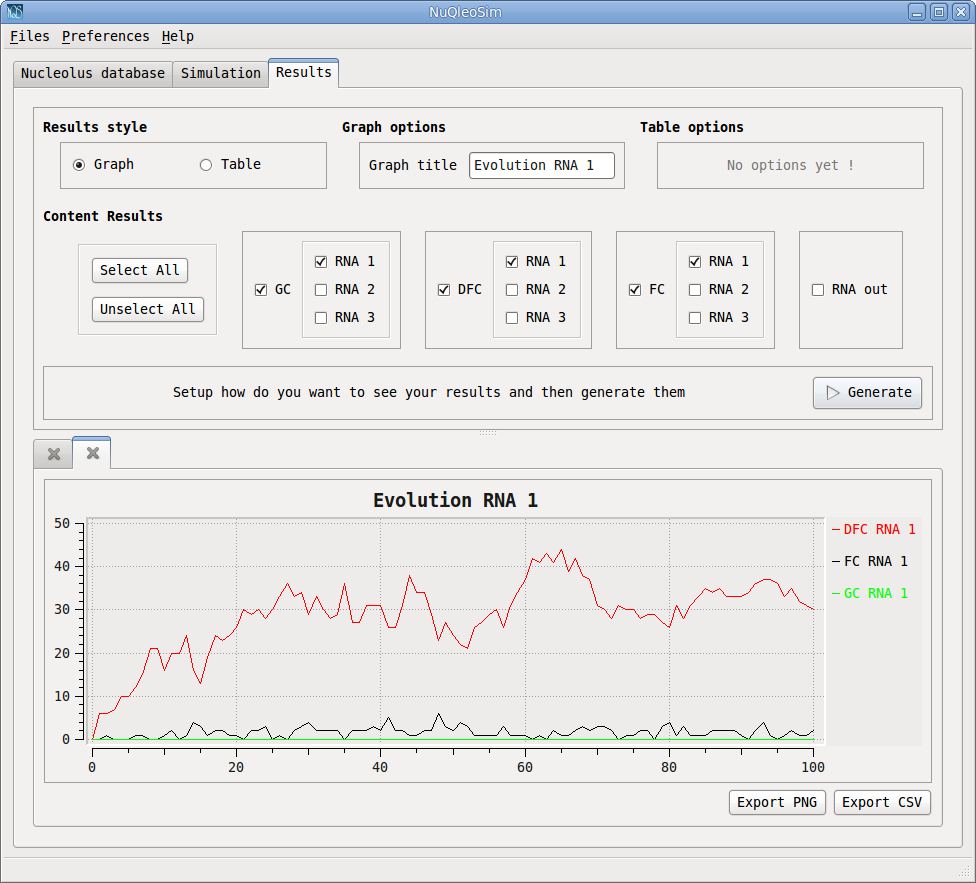
\includegraphics[width=0.7\columnwidth]{img/inter4.png}
    \end{center}
\end{frame}

%%%%%%%%%%%%%%%%%%%%%%%%%%%%%%%%%%%%%%%%%%%%%%%%%%%%%%%%%%%%%%%%%%%%%%%%%%%%%%%%%%%%%%%%%%%%

\section*{Conclusion}

\begin{frame}
  \frametitle{Conclusion}

  \begin{block}{Fonctionalités de NuQleoSim}
    \begin{itemize}
    \item Construction, exploitation et gestion d'une BD
    \item Simulation paramétrable en liaison avec la BD
    \item Visualisation de la simulation en temps réel
    \item Présentation paramétrable des résultats
    \end{itemize}
  \end{block}
  \begin{block}{Perspectives d'amélioration}
    \begin{itemize}
    \item Base de données interchangeable
    \item Simulation remplaçable
    \item Exploitation des résultats maléable
    \end{itemize}
  \end{block}
\end{frame}

%%%%%%%%%%%%%%%%%%%%%%%%%%%%%%%%%%%%%%%%%%%%%%%%%%%%%%%%%%%%%%%%%%%%%%%%%%%%%%%%%%%%%%%%%%%%%%%%%%%

\begin{frame}
\begin{center}

\includegraphics[width=0.3\columnwidth]{img/merci.png}
\end{center}
\begin{center}pour votre attention\end{center}
\end{frame}

\end{document}

